\begin{figure}[t]
	\centering
	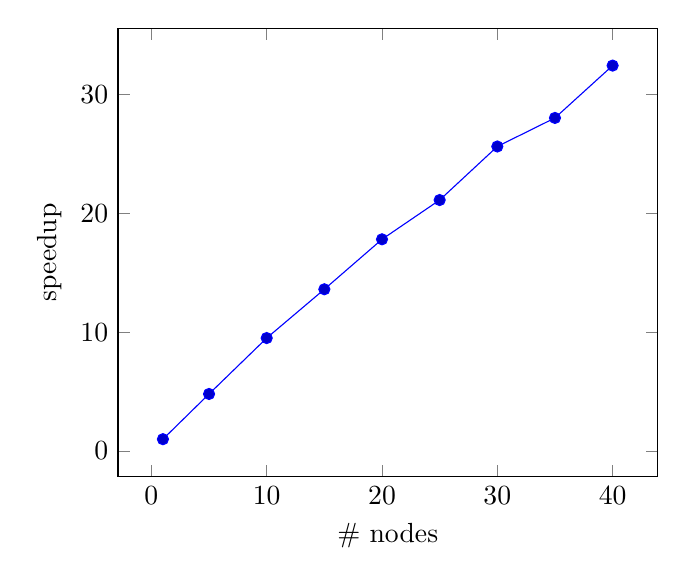
\begin{tikzpicture}
	\begin{axis}[xlabel=\# nodes,ylabel=speedup]
	\addplot coordinates {
		(1, 1)
		(5, 4.8)
		(10, 9.5)
		(15, 13.6)
		(20, 17.8)
		(25, 21.1)
		(30, 25.6)
		(35, 28.0)
		(40, 32.4)
	};
	\end{axis}
	\end{tikzpicture}
	\caption{Observed speedup when traversing the GIT fan with varying numbers of compute nodes.}
	\label{graph:traversal_speedup}
\end{figure}

\begin{figure}[t]
	\centering
	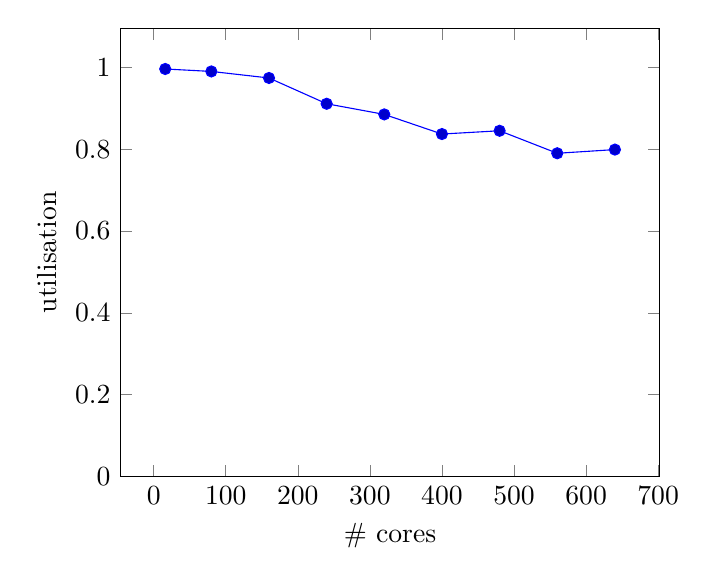
\begin{tikzpicture}
	\begin{axis}[xlabel=\# cores,ylabel=utilisation,ymin=0]
	\addplot coordinates {
		(16, 0.996)
		(80, 0.990)
		(160, 0.974)
		(240, 0.911)
		(320, 0.885)
		(400, 0.837)
		(480, 0.845)
		(560, 0.790)
		(640, 0.799)
	};
	\end{axis}
	\end{tikzpicture}
	\caption{Observed utilisation when traversing the GIT fan with varying numbers of compute nodes.}
	\label{graph:traversal_utilisation}
\end{figure}

\begin{figure}[t]
	\centering
	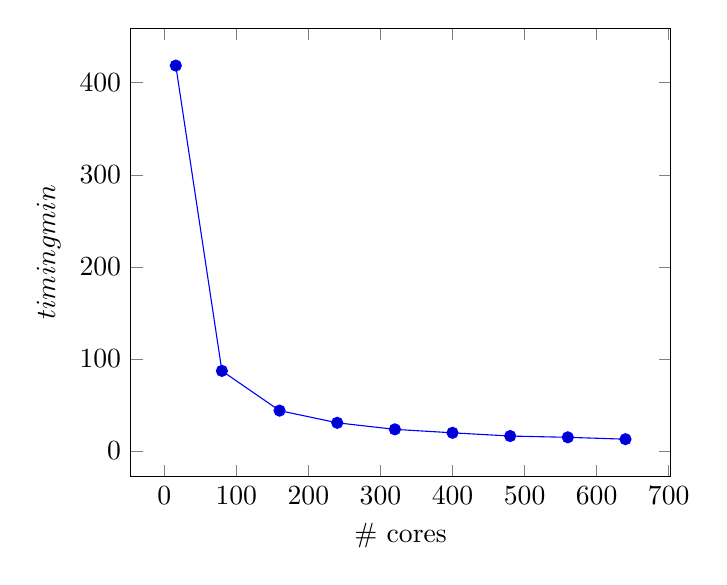
\begin{tikzpicture}
	\begin{axis}[xlabel=\# cores,ylabel=$\faktor{\text{timing}}{\text{min}}$]
	\addplot coordinates {
		(16, 418.5950)
		(80, 87.0672)
		(160, 43.9218)
		(240, 30.6985)
		(320, 23.5702)
		(400, 19.8228)
		(480, 16.3206)
		(560, 14.9239)
		(640, 12.9088)
	};
	\end{axis}
	\end{tikzpicture}
	\caption{Required computation time when traversing the GIT fan with varying numbers of compute nodes.}
	\label{graph:traversal_timing}
\end{figure}